% -*- TeX -*- -*- UK -*- -*- Soft -*-

\chapter{Understanding Bayes}
\label{chap:UnderstandingBayes}


Taken verbatim from \cite{etz2015a,etz2015d,etz2015b,etz2015c,etz2016a}.

\section{A Look at the Likelihood}
\label{sec:ALookattheLikelihood}

Much of the discussion in psychology surrounding Bayesian inference focuses on priors. Should we embrace priors, or should we be skeptical? When are Bayesian methods sensitive to specification of the prior, and when do the data effectively overwhelm it? Should we use context specific prior distributions or should we use general defaults? These are all great questions and great discussions to be having.

One thing that often gets left out of the discussion is the importance of the likelihood. The likelihood is the workhorse of Bayesian inference. In order to understand Bayesian parameter estimation you need to understand the likelihood. In order to understand Bayesian model comparison (Bayes factors) you need to understand the likelihood and likelihood ratios.

\subsection{What is likelihood?}

Likelihood is a funny concept. It's not a probability, but it is \textit{proportional} to a probability. The likelihood of a hypothesis ($H$) given some data ($D$) is proportional to the probability of obtaining $D$ given that $H$ is true, multiplied by an arbitrary positive constant ($K$). In other words, $\mathrm{L}(\mathrm{H} | \mathrm{D})=\mathrm{K} \cdot \mathrm{P}(\mathrm{D} | \mathrm{H})$. Since a likelihood isn't actually a probability it doesn't obey various rules of probability. For example, likelihood need not sum to 1.

A critical difference between probability and likelihood is in the interpretation of what is fixed and what can vary. In the case of a conditional probability, $\mathrm{P}(\mathrm{D} | \mathrm{H})$, the hypothesis is fixed and the data are free to vary. Likelihood, however, is the opposite. The likelihood of a hypothesis, $\mathrm{L}(\mathrm{H} | \mathrm{D})$, conditions on the data as if they are fixed while allowing the hypotheses to vary.

The distinction is subtle, so I'll say it again. For conditional probability, the hypothesis is treated as a given and the data are free to vary. For likelihood, the data are a given and the hypotheses vary.
The Likelihood Axiom

Edwards \cite[p 30]{Edwards1992} defines the Likelihood Axiom as a natural combination of the Law of Likelihood and the Likelihood Principle.

The \textbf{Law of Likelihood} states that ''within the framework of a statistical model, a particular set of data supports one statistical hypothesis better than another if the likelihood of the first hypothesis, on the data, exceeds the likelihood of the second hypothesis'' (Emphasis original, \cite[p 30]{Edwards1992}).

In other words, there is evidence for $H1$ vis-a-vis $H2$ if and only if the probability of the data under $H1$ is greater than the probability of the data under $H2$. That is, $D$ is evidence for $H1$ over $H2$ if $\mathrm{P}(\mathrm{D} | \mathrm{H} 1)>\mathrm{P}(\mathrm{D} | \mathrm{H} 2)$. If these two probabilities are equivalent, then there is no evidence for either hypothesis over the other. Furthermore, the strength of the statistical evidence for $H1$ over $H2$ is quantified by the ratio of their likelihoods, $\mathrm{L}(\mathrm{H} 1 | \mathrm{D}) / \mathrm{L}(\mathrm{H} 2 | \mathrm{D})$ (which again is proportional to $\mathrm{P}(\mathrm{D} | \mathrm{H} 1) / \mathrm{P}(\mathrm{D} | \mathrm{H} 2)$ up to an arbitrary constant that cancels out).

The \textbf{Likelihood Principle} states that the likelihood function contains all of the information relevant to the evaluation of statistical evidence. Other facets of the data that do not factor into the likelihood function are \textit{irrelevant} to the evaluation of the strength of the statistical evidence 
\cite[p 30]{Edwards1992},cite[p 22]{Royall2000}. They can be meaningful for planning studies or for decision analysis, but they are separate from the 
\textit{strength} of the statistical evidence.

\subsection{Likelihoods are meaningless in isolation}

Unlike a probability, a likelihood has no real meaning \textit{per se} due to the arbitrary constant. Only by comparing likelihoods do they become interpretable, because the constant in each likelihood cancels the other one out. The easiest way to explain this aspect of likelihood is to use the binomial distribution as an example.

Suppose I flip a coin 10 times and it comes up 6 heads and 4 tails. If the coin were fair, p(heads) = .5, the probability of this occurrence is defined by the binomial distribution:
\begin{equation}
P(X=x)=
\left(\begin{array}{l}
n \\x\end{array}\right) 
p^{x}(1-p)^{n-x}
\end{equation}
where $x$ is the number of heads obtained, $n$ is the total number of flips, $p$ is the probability of heads, and
\begin{equation}
\left(\begin{array}{l}
n \\x\end{array}\right)
=\frac{n !}{x !(n-x) !}
\end{equation}
Substituting in our values we get
\begin{equation}P(X=6)=\frac{10 !}{6 !(4 !)}(.5)^{6}(1-.5)^{4} \approx .21\end{equation}
If the coin were a trick coin, so that p(heads) = .75, the probability of 6 heads in 10 tosses is:
\begin{equation}P(X=6)=\frac{10 !}{6(4 ! !)}(.75)^{6}(1-.75)^{4} \approx .15\end{equation}
To quantify the statistical evidence for the first hypothesis against the second, we simply divide one probability by the other. This ratio tells us everything we need to know about the support the data lends to one hypothesis vis-a-vis the other.  In the case of 6 heads in 10 tosses, the likelihood ratio (LR) for a fair coin vs our trick coin is:
\begin{equation}L R=\left(\frac{10 !}{6 !(4 !)}(.5)^{6}(1-.5)^{4}\right) \div\left(\frac{10 !}{6 !(4 !)}(.75)^{6}(1-.75)^{4}\right) \approx .21 / .15 \approx 1.4\end{equation}
Translation: The data are 1.4 times as probable under a fair coin hypothesis than under this particular trick coin hypothesis. Notice how the first terms in each of the equations above, i.e., $\frac{10 !}{6 !(4 !)}$ , are equivalent and completely cancel each other out in the likelihood ratio.

\textsl{Same data. Same constant. Cancel out.}

The first term in the equations above, $\frac{10 !}{6 !(4 !)}$, details \textit{our journey} to obtaining 6 heads out of 10. If we change our journey (i.e., different sampling plan) then this changes the term's value, \textbf{but crucially, since it is the same term in both the numerator and denominator it always cancels itself out}. In other words, the information contained in the way the data are obtained \textit{disappears from the function}. Hence the irrelevance of the stopping rule to the evaluation of statistical evidence, which is something that makes bayesian and likelihood methods valuable and flexible.

If we leave out the first term in the above calculations, our numerator is $L(.5)=0.0009765625$
 and our denominator is $\mathrm{L}(.75) \approx 0.0006952286$. Using these values to form the likelihood ratio we get: $0.0009765625 / 0.0006952286 \approx 1.4$, as we should since the other terms simply cancelled out before.

Again I want to reiterate that the value of a single likelihood is meaningless in isolation; only in \textit{comparing} likelihoods do we find meaning.

\subsection{Looking at likelihoods}

Likelihoods may seem overly restrictive at first. We can only compare 2 simple statistical hypotheses in a single likelihood ratio. But what if we are interested in comparing many more hypotheses at once? What if we want to compare all possible hypotheses at once?

In that case we can plot the likelihood function for our data, and this lets us ‘see' the evidence in its entirety. By plotting the entire likelihood function we compare all possible hypotheses simultaneously. The Likelihood Principle tells us that the likelihood function encompasses all statistical evidence that our data can provide, so we should always plot this function along side our reported likelihood ratios.

Following the wisdom of Birnbaum \cite{Birnbaum1962}, ''the ''evidential meaning'' of experimental results is characterized fully by the likelihood function'' (as cited in \cite[p 25]{Royall2000}). So let's look at some examples. The R script at the end of this post can be used to reproduce these plots, or you can use it to make your own plots. Play around with it and see how the functions change for different number of heads, total flips, and hypotheses of interest. See the instructions in the script for details.

The graph shows the likelihood function for 6 heads in 10 tosses. I've marked our two hypotheses from before on the likelihood curve with blue dots. Since the likelihood function is meaningful only up to an arbitrary constant, the graph is scaled by convention so that the best supported value (i.e., the maximum) corresponds to a likelihood of 1.

\begin{figure}[h]
    \centering
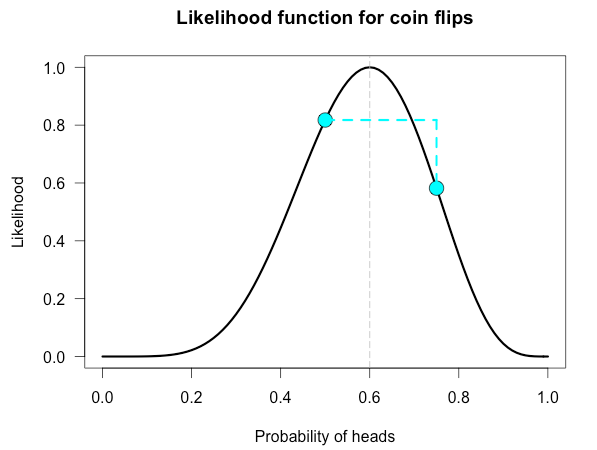
\includegraphics[width=0.8\textwidth]{pic/p05c03-snip01.png}
    \caption{Likelihood function for 6 heads in 10 flips}
    \label{fig:p05c03-snip01}
\end{figure}

The vertical dotted line marks the hypothesis best supported by the data. The likelihood ratio of any two hypotheses is simply the ratio of their heights on this curve. We can see from the plot that the fair coin has a higher likelihood than our trick coin.

How does the curve change if instead of 6 heads out of 10 tosses, we tossed 100 times and obtained 60 heads?

\begin{figure}[h]
    \centering
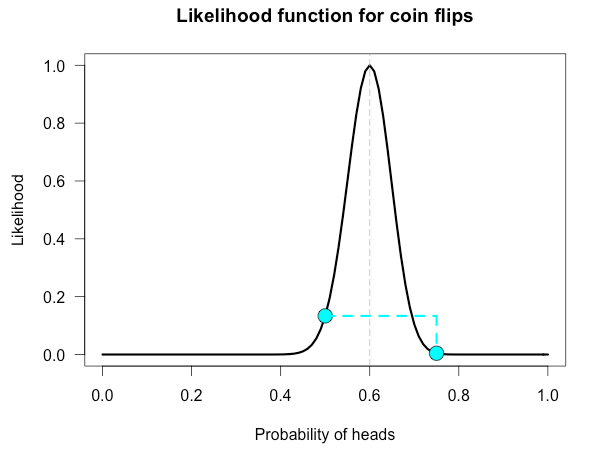
\includegraphics[width=.8\textwidth]{pic/p05c03-snip02.png}
    \caption{Likelihood function for  60 heads in 100  flips}
    \label{fig:p05c03-snip02}
\end{figure}

Our curve gets much narrower! How did the strength of evidence change for the fair coin vs the trick coin? The new likelihood ratio is $\mathrm{L}(.5) / \mathrm{L}(.75) \approx 29.9$. Much stronger evidence!\footnote{Obtaining 60 heads in 100 tosses is equivalent to obtaining 6 heads in 10 tosses 10 separate times. To obtain this new likelihood ratio we can simply multiply our ratios together. That is, raise the first ratio to the power of 10; $1.4^{\wedge} 10 \approx 28.9$, which is just slightly off from the correct value of 29.9 due to rounding.} However, due to the narrowing, neither of these hypothesized values are very high up on the curve anymore. It might be more informative to compare each of our hypotheses against the best supported hypothesis. This gives us two likelihood ratios: $\mathrm{L}(.6) / \mathrm{L}(.5) \approx 7.5$  and $\mathrm{L}(.6) / \mathrm{L}(.75) \approx 224$.

\begin{figure}[h]
    \centering
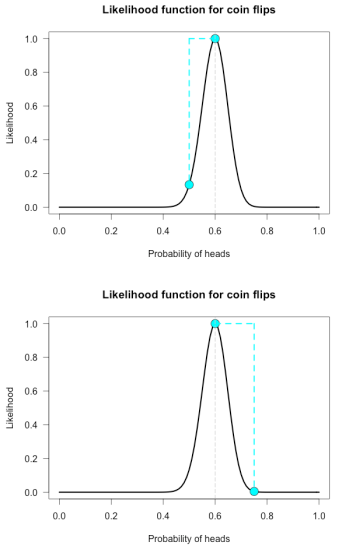
\includegraphics[width=0.8\textwidth]{pic/p05c03-snip03.png}
    \caption{Likelihood function ratios 7.5 and 224}
    \label{fig:p05c03-snip03}
\end{figure}

Here is one more curve, for when we obtain 300 heads in 500 coin flips.

\begin{figure}[h]
    \centering
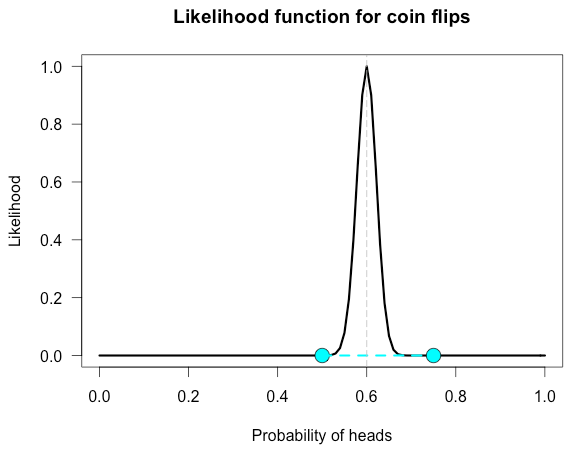
\includegraphics[width=0.8\textwidth]{pic/p05c03-snip04.png}
    \caption{Likelihood function for  300 heads in 500  flips}
    \label{fig:p05c03-snip04}
\end{figure}

Notice that both of our hypotheses look to be very near the minimum of the graph. Yet their likelihood ratio is much stronger than before. For this data the likelihood ratio$\mathrm{L}(.5) / \mathrm{L}(.75)$ is nearly \textbf{24 million!} The inherent relativity of evidence is made clear here: The fair coin was supported when compared to \textit{one particular} trick coin. But this should not be interpreted as absolute evidence for the fair coin, because the likelihood ratio for the maximally supported hypothesis vs the fair coin, $\mathrm{L}(.6) / \mathrm{L}(.5)$, is nearly \textbf{24 thousand!}

We need to be careful not to make blanket statements about absolute support, such as claiming that the maximum is ''strongly supported by the data''. Always ask, ''Compared to what?'' The best supported hypothesis will be only be weakly supported vs any hypothesis just before or just after it on the x-axis. For example, $\mathrm{L}(.6) / \mathrm{L}(.61) \approx 1.1$, which is barely any support one way or the other. It cannot be said enough that evidence for a hypothesis must be evaluated in consideration with a specific alternative.

\subsection{Connecting likelihood ratios to Bayes factors}

Bayes factors are simple extensions of likelihood ratios. A Bayes factor is a weighted average likelihood ratio based on the prior distribution specified for the hypotheses. (When the hypotheses are simple point hypotheses, the Bayes factor is equivalent to the likelihood ratio.) The likelihood ratio is evaluated at each point of the prior distribution and weighted by the probability we assign that value. If the prior distribution assigns the majority of its probability to values far away from the observed data, then the average likelihood for that hypothesis is lower than one that assigns probability closer to the observed data. In other words, you get a Bayes boost if you make more accurate predictions. Bayes factors are extremely valuable, and in a future post I will tackle the hard problem of assigning priors and evaluating weighted likelihoods.

I hope you come away from this post with a greater knowledge of, and appreciation for, likelihoods. Play around with the R code and you can get a feel for how the likelihood functions change for different data and different hypotheses of interest.


\begin{lstlisting}
## R code for th plots
## Plots the likelihood function for the data obtained
## h = number of successes (heads), n = number of trials (flips), 
## p1 = prob of success (head) on H1, p2 = prob of success (head) on H2
## Returns the likelihood ratio for p1 over p2. The default values are the ones used in the blog post
LR <- function(h,n,p1=.5,p2=.75){
        L1 <- dbinom(h,n,p1)/dbinom(h,n,h/n) ## Likelihood for p1, standardized vs the MLE
        L2 <- dbinom(h,n,p2)/dbinom(h,n,h/n) ## Likelihood for p2, standardized vs the MLE
        Ratio <- dbinom(h,n,p1)/dbinom(h,n,p2) ## Likelihood ratio for p1 vs p2
        curve((dbinom(h,n,x)/max(dbinom(h,n,x))), xlim = c(0,1), ylab = "Likelihood",xlab = "Probability of heads",las=1,
                main = "Likelihood function for coin flips", lwd = 3)
        points(p1, L1, cex = 2, pch = 21, bg = "cyan")
        points(p2, L2, cex = 2, pch = 21, bg = "cyan")
        lines(c(p1, p2), c(L1, L1), lwd = 3, lty = 2, col = "cyan")
        lines(c(p2, p2), c(L1, L2), lwd = 3, lty = 2, col = "cyan")
        abline(v = h/n, lty = 5, lwd = 1, col = "grey73")
        return(Ratio) ## Returns the likelihood ratio for p1 vs p2
}
\end{lstlisting}

(footnote) Obtaining 60 heads in 100 tosses is equivalent to obtaining 6 heads in 10 tosses 10 separate times. To obtain this new likelihood ratio we can simply multiply our ratios together. That is, raise the first ratio to the power of 10; $1.4^{\wedge} 10 \approx 28.9$, which is just slightly off from the correct value of 29.9 due to rounding.

In the comments to the above blog, someone wrote:
`` Bayesian statistics is a religion that gives a false promise of certainty to believers in a world of uncertainty.''

\section{Updating priors via the likelihood}
\label{sec:Updatingpriorsviathelikelihood}




\section{Visualization of the Bayes Factor}
\label{sec:VisualizationoftheBayesFactor}



\section{Evidence vs. Conclusions}
\label{sec:Evidencevs.Conclusions}



\section{How to become a Bayesian in eight easy steps}
\label{sec:HowtobecomeaBayesianineighteasysteps}




